\chapter{Análisis espectrales: resultados numéricos}
\label{chap: resultados numericos analisis espectrales}

\TODO{Agrega intro.}

Programando la funciones necesarias para realizar análisis espectrales
usando estas dos metodologías, podremos comprobar o refutar y mejorar
la hipótesis hecha en 
\ref{ref: hipotesis}. 
Escribimos en la siguiente sección unas preguntas guía
que nos gustaría responder numéricamente, después de 
realizar análisis espectrales de los PDL
$\cali{L}^{n,k}$ de dimensión $2 \leq 2 \leq 69$. \\

No realizamos el análisis espectral para dimensiones
mayores a $69$ pues, para dimensiones más grandes, los números
involucrados en los cálculos son tan pequeños
en magnitud que son redondeados a cero
\sidenote{Puede consultar \cite{DSmath} para ver los detalles de cómo los
datos de tipo \texttt{float} son manipulados por la computadora
y los problemas de aproximación y redondeo que están implícitos en
este tipo de operaciones.}

\TODO{Dí que se ve que un espectro está contenido en el otro y 
cita la proposición \ref{prop: coinciden espectr}.}

\section{Preguntas a responder numéricamente sobre las oscilaciones de los PDL}

Enlistamos las preguntas que nos interesa considerar
relacionadas a las naturaleza oscilatoria
de los PDL $\cali{L}^{n,k}$
para dimensiones hasta $n=69$. 

La primera pregunta es una reformulación de la 
hipótesis \ref{ref: hipotesis} en términos de los 
valores $FM0(x)$ y $FM1(x)$ definidos en 
\ref{def: FM0} y \ref{def: FM1}.

\begin{pregunta}
\label{pregunta 1}
Sean $2 \leq n \leq 69$ y $0 \leq k \leq n-1$.
Sea $\cali{L}^{n,k}$ el PDL de dimensión $n$ y grado $k$.
¿las frecuencias máximas
$FM0(\cali{L}^{n,k})$ y 
$FM1(\cali{L}^{n,k})$ son cercanas a $\frac{k}{2}$?
\end{pregunta}

A continuación mostramos un dibujo para
ilustrar cómo podrían verse los
espectros del PDL
$\cali{L}^{7,5} \in \IR^{7}$
en caso de que la respuesta a la pregunta
\ref{pregunta 1} sea afirmativa.
Se escogió dibujar posibles espectros
de $\cali{L}^{7,5}$; observe que, en el segundo espectro,
fue posible usar varios valores de $\omega$ para analizar
a $\cali{L}^{7,5}$, y que podría ser que la frecuencia máxima
sea un número decimal, mientras que para el primer espectro
(el basado en la TDF) sólo pueden usarse algunas frecuencias
enteras, por lo que no esperamos que el valor máximo
se de en $\frac{5}{2}$, pues este ni siquiera es un entero.
Esperamos, sin embargo, que el máximo se de en las frecuencias
enteras cercanas al valor $\frac{5}{2}$.

\begin{figure}[H]
	\sidecaption{
	A la izquierda un dibujo (no basado en datos reales) de 
	un posible espectro para $\cali{L}^{n,k}$ basado en la 
	DFT, y a la derecha uno basado en cosenos a espacios 
	monofrecuenciales. Observe que en el segundo espectro se pueden
	considerar muchas más frecuencias que en el primero.
	\label{fig: ejemplo_pregunta1}
	}
	\centering
	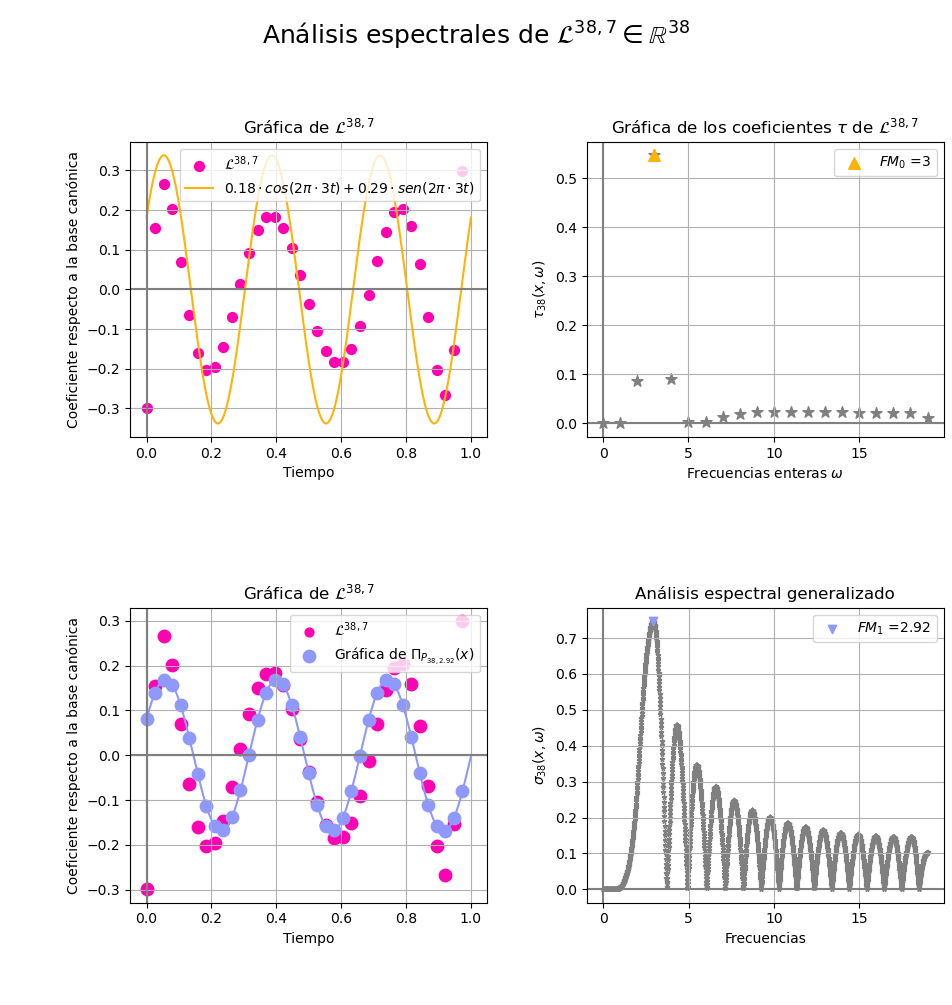
\includegraphics[scale = 0.9]{./estudios_espectrales/ejemplo_pregunta1} 
\end{figure}	

\begin{pregunta}
\label{preg 2}
¿Las frecuencias 
$FM0(\cali{L}^{n,k})$ y $FM1(\cali{L}^{n,k})$
dependen, como implica la pregunta 1, sólo del parámetro
de grado $k$ y no del de dimensión $n$?
Es decir, si $k$, $n_{1}$ y $n_{2}$
son tales que $k \leq n_{1}-1$ y
$k \leq n_{2}-1$, ¿ocurre que 
$FM0(\cali{L}^{n_{1},k})$ = $FM0(\cali{L}^{n_{2},k})$
y 
$FM1(\cali{L}^{n_{1},k})$ = $FM1(\cali{L}^{n_{2},k})$?
\end{pregunta}

Para tratar de responder a la pregunta \ref{preg 2},
fijado un grado $k$,
podría ser útil graficar los puntos de la forma
\[
(n, FM0(\cali{L}^{n,k})), \hspace{0.2cm} k < n \leq 69,
\] y 
\[
(n, FM1(\cali{L}^{n,k})), \hspace{0.2cm} k < n \leq 69.
\]
Gráficas de este estilo podrían usarse para comprobar
la respuesta a la pregunta \ref{pregunta 1} 
graficando también la recta horizontal $y = \frac{k}{2}$
y viendo si los puntos graficados se encuentran cerca
de esta recta o no.

\begin{figure}[H]
	\sidecaption{
	 De ser la respuesta
	a la pregunta \ref{preg 2} afirmativa, deberíamos
	de terminar con gráficas de puntos alineados horizontalmente, como
	en este dibujo. Sería bueno que los puntos $FM0$ y $FM1$ estuviesen
	a alturas parecidas, pues eso significaría que los dos análisis espectrales
	dan resultados parecidos.
	\label{fig: ejemplo_pregunta2}
	}
	\centering
	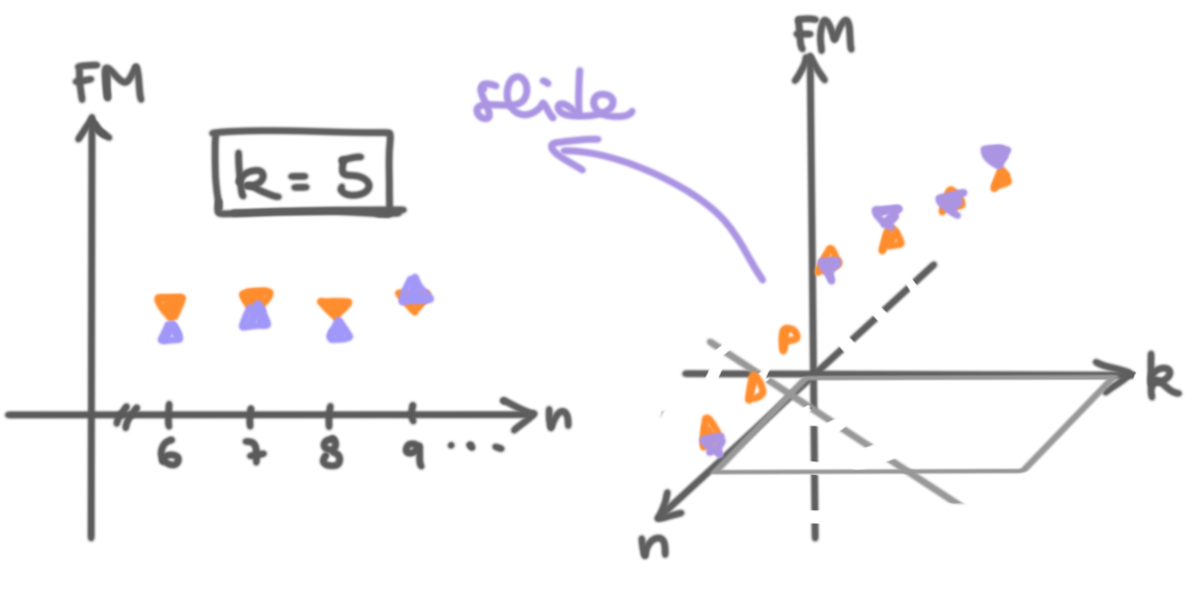
\includegraphics[scale = 1.4]{./estudios_espectrales/ejemplo_pregunta2} 
\end{figure}	

\begin{pregunta}
\label{preg 3}
Fijada una dimensión $2 \leq n \leq 69$,
considere las gráficas de los
puntos 
\begin{equation}
\label{eq5: May1}
(k, FM0(\cali{L}^{n,k})), \hspace{0.2cm} 0 \leq k \leq n-1
\end{equation}
y
\begin{equation}
\label{eq6: May1}
(k, FM1(\cali{L}^{n,k})), \hspace{0.2cm} 0 \leq k \leq n-1,
\end{equation}

\noindent
o sea, las gráficas de las frecuencias máximas encontradas
en los dos análisis espectrales para cada
PDL de dimensión $n$.
Sean $m_{n,0}$ y $b_{n,0}$ la pendiente y la ordenada
al origen de la recta de mínimos cuadrados calculada a 
partir del conjunto de puntos 
\eqref{eq5: May1}, y
$m_{n,1}$ y $b_{n,1}$ los correspondientes parámetros
para el conjunto de puntos 
\eqref{eq6: May1}.

Considere las nubes de puntos 
\[
(b_{n,0}, m_{n,0}), \hspace{0.2cm} 2 \leq n \leq 69
\]
y 
\[
(b_{n,1}, m_{n,1}), \hspace{0.2cm} 2 \leq n \leq 69.
\]
¿Alrededor de qué punto parecen concentrarse estas nubes?
\end{pregunta}

Investigar la respuesta (numéricamente)
de esta última pregunta nos ayudará a afinar 
la estimación de frecuencias establecida
en la pregunta \ref{pregunta 1}. 

\begin{figure}[H]
	\sidecaption{
	Se muestran las gráficas 
	de las colecciones de puntos
	\eqref{eq5: May1} y \eqref{eq6: May1}
	para $n=7$	
	descritas en la pregunta
	\ref{preg 3}.
	\label{fig: ejemplo_pregunta3_0}
	}
	\centering
	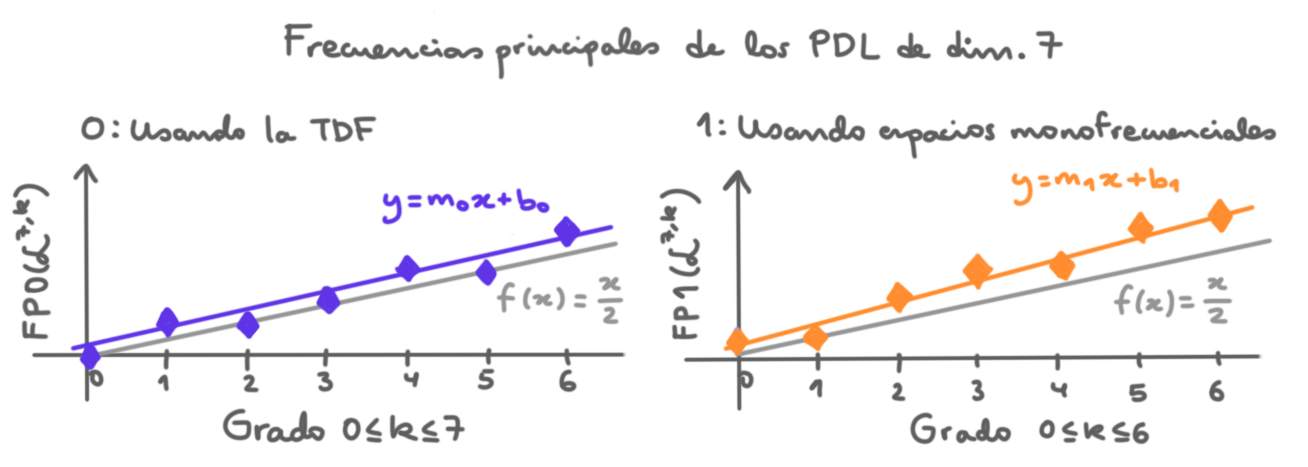
\includegraphics[scale = 1.1]{./estudios_espectrales/ejemplo_pregunta3_0} 
\end{figure}	

\begin{figure}[H]
	\sidecaption{
	Si la estimación dada en la pregunta \ref{pregunta 1} es
	buena, las nubes de puntos descritas en la 
	pregunta \ref{preg 3} deberían estar centradas
	en el punto $(0, 0.5)$.
	\label{fig: ejemplo_pregunta3_1}
	}
	\centering
	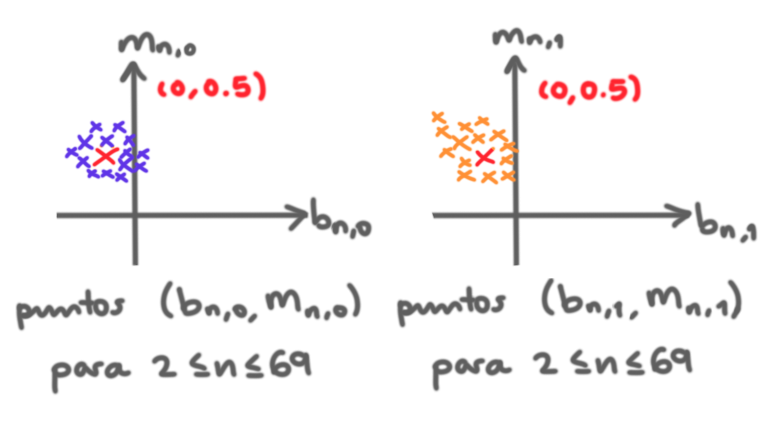
\includegraphics[scale = 1.5]{./estudios_espectrales/ejemplo_pregunta3} 
\end{figure}	


Vamos a responder a estas preguntas con gráficas parecidas
a las dibujadas en las figuras
\ref{fig: ejemplo_pregunta1},
\ref{fig: ejemplo_pregunta2},
\ref{fig: ejemplo_pregunta3_0} y
\ref{fig: ejemplo_pregunta3_1}.

Vamos a responder a la pregunta \ref{pregunta 1} graficando
algunos espectros y comprobando si las
frecuencias $FM0(\cali{L}^{n,k})$ y 
$FM1(\cali{L}^{n,k})$ son, en efecto, cercanas a $\frac{k}{2}$.

Para calcular los datos necesarios para responder
las preguntas \ref{preg 2} y \ref{preg 3},
usando la función \texttt{analisis$\_$espectralPDL$\_$global(n)}, 
para toda dimensión
$2 \leq n \leq 69$ calculamos
\begin{itemize}
	\item los coeficientes $FM1(\cali{L}^{n,k})$ para toda
	$0 \leq k \leq n-1$, y guardamos esta información en el
	array \texttt{sigmasMax$\_$n},
	\item los coeficientes $FM0(\cali{L}^{n,k})$ para toda
	$0 \leq k \leq n-1$, y guardamos esta información en el
	array \texttt{tausMax$\_$n},
	\item y los números $b_{n,0}$, $m_{n,0}$,
	$b_{n,1}$ y $m_{n,1}$ como se definieron en la pregunta
	\ref{preg 3}.
\end{itemize}
Toda esta información se calculó una sola vez y se almacenó
en un diccionario, cuyas llaves son las dimensiones
$n$, y cuyo valor asociado a la llave $n$ es la $6-$tupla
\[
(sigmasMax\_n, tausMax\_n, b_{n,0}, m_{n,0}, b_{n,1}, m_{n,1}).
\]

\begin{figure}[H]
	\sidecaption{
	En la figura de la izquierda se grafican los
	puntos $(b_{0,n}, m_{0, n})$, siendo la primera entrada
	la ordenada al origen de la recta de mínimos cuadrados
	de \TODO{ref} y la segunda entrada la pendiente de esta.
	\label{fig: pendiente_oOrigen}
	}
	\centering
	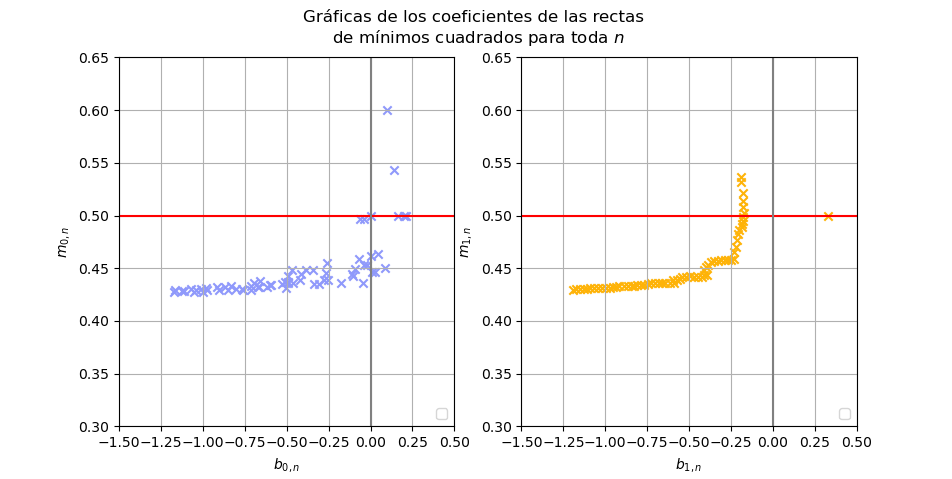
\includegraphics[scale = 0.6]{./estudios_espectrales/pendiente_oOrigen} 
\end{figure}	

Los códigos, escritos en Python, pueden encontrase en 
\TODO{referencia al repositorio.} Usamos el 
módulo \texttt{pickle} para guardar los datos como secuencias
de bytes. El archivo binario en el que se almacenaron los
datos calculados con la función 
\texttt{analisis$\_$espectralPDL$\_$global(n)}
es \TODO{ref}.

\section{Gráficas para la pregunta \ref{pregunta 1}}


\section{Gráficas para la pregunta \ref{preg 2}}

\section{Gráficas para la pregunta \ref{preg 3}}

\begin{figure}[H]
	\sidecaption{
	\label{fig: tablas_1,2}
	}
	\centering
	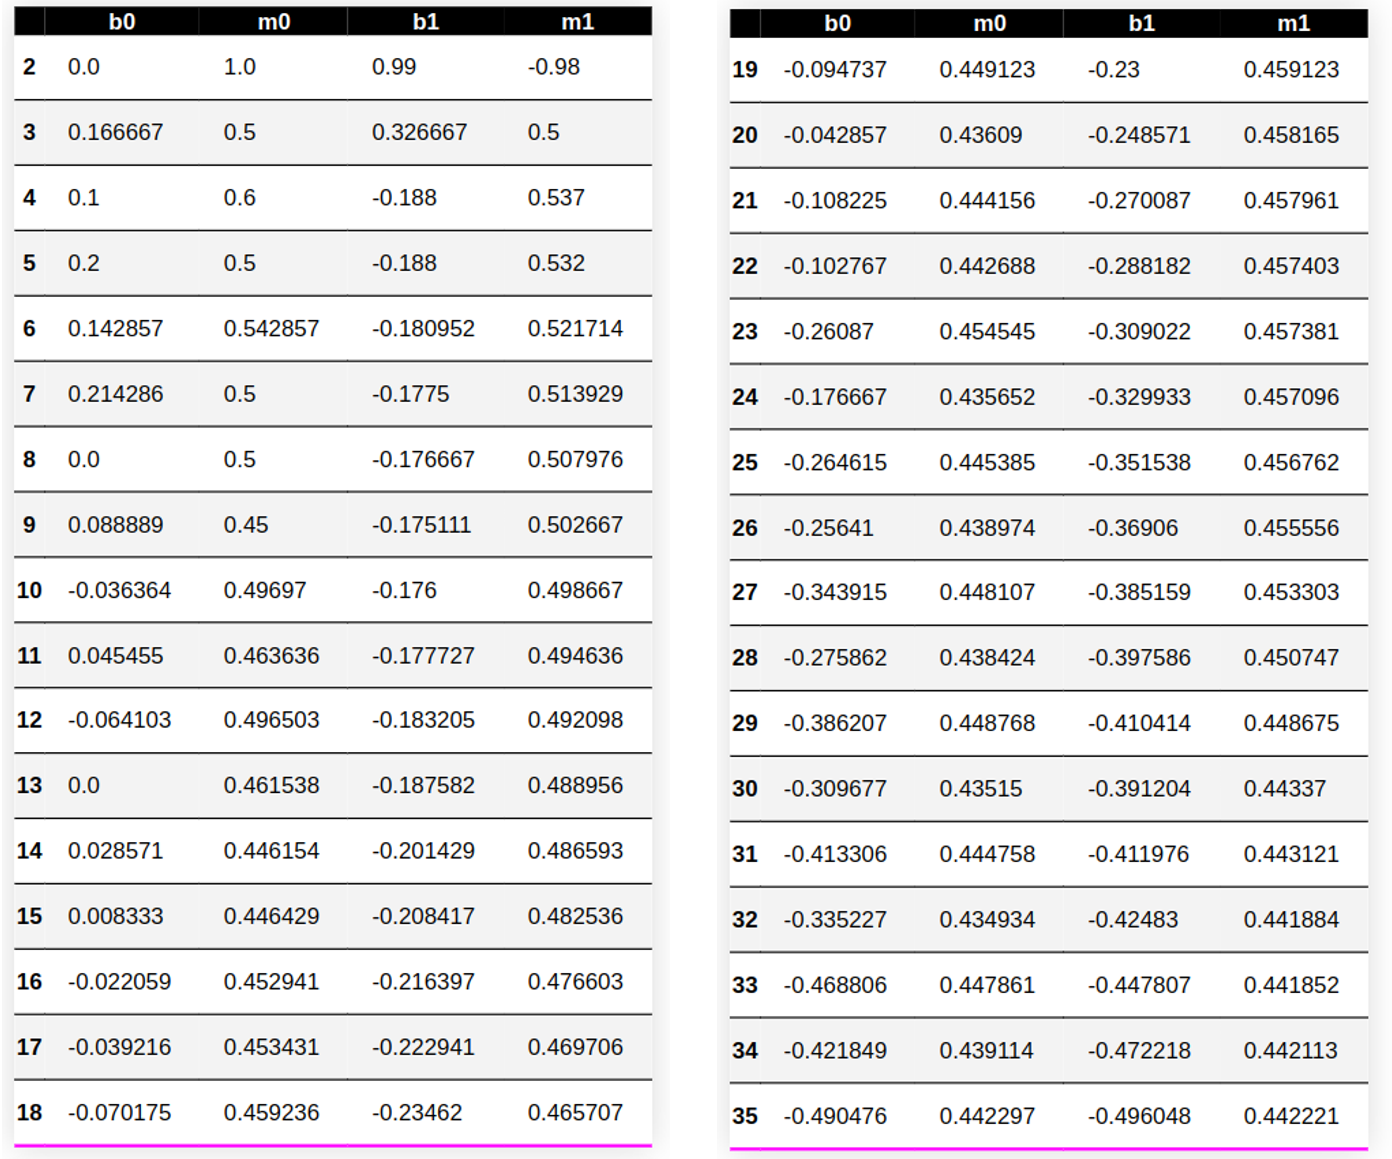
\includegraphics[scale = 1.1]{./estudios_espectrales/tablas_1,2} 
\end{figure}	

\begin{figure}[H]
	\sidecaption{
	\label{fig: tablas_1,2}
	}
	\centering
	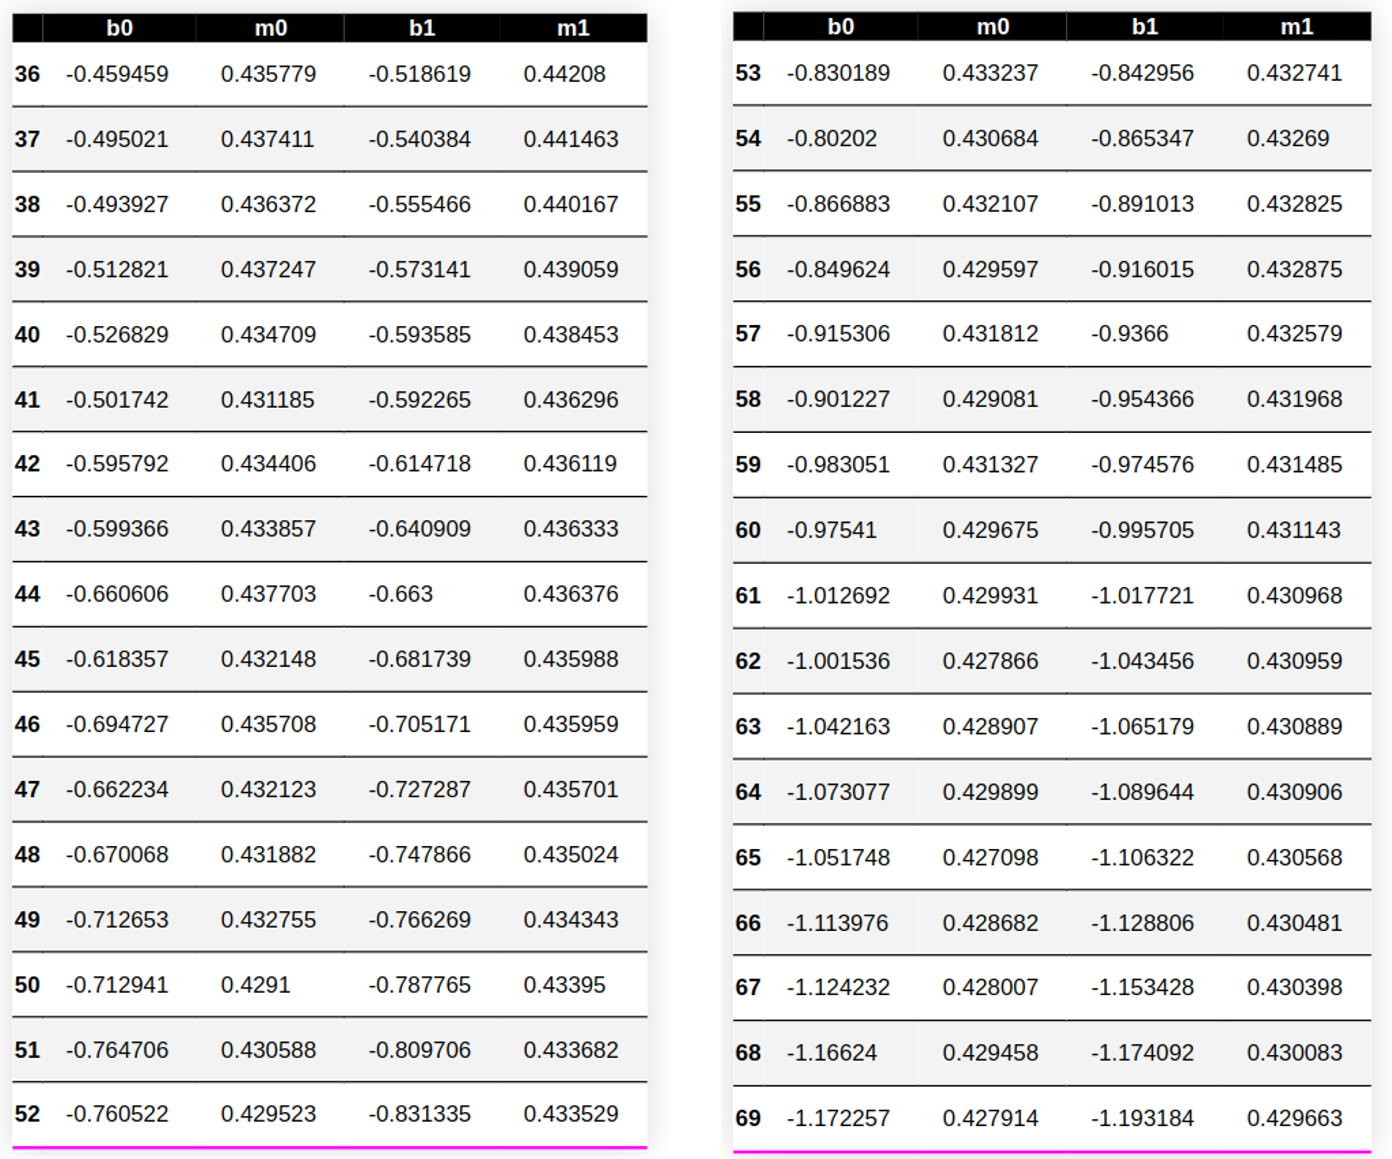
\includegraphics[scale = 1.1]{./estudios_espectrales/tablas_3,4} 
\end{figure}	